\documentclass{article}
\usepackage{tikz}
\usetikzlibrary{arrows.meta}

\begin{document}

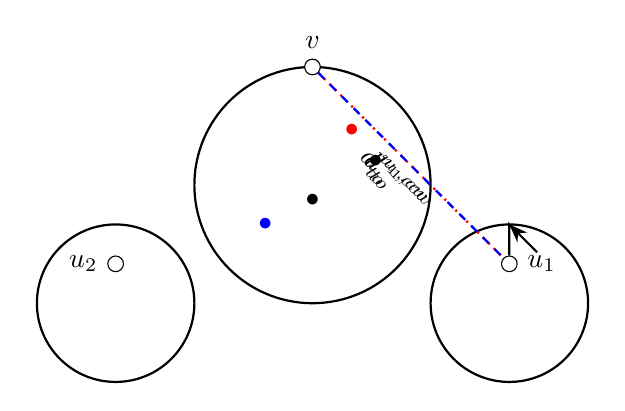
\begin{tikzpicture}[dot/.style={circle, draw=black, fill=white, inner sep=2pt}, >=Stealth]
    % Draw the outer circle
    \draw[thick] (0,0) circle (1.5cm);
    
    % Draw the smaller circles
    \draw[thick] (-2.5,-1.5) circle (1cm);
    \draw[thick] (2.5,-1.5) circle (1cm);
    
    % Label the vertices
    \node[dot,label=above:$v$] (v) at (0,1.5) {};
    \node[dot,label=left:$u_2$] (u2) at (-2.5,-1) {};
    \node[dot,label=right:$u_1$] (u1) at (2.5,-1) {};
    
    % Draw the paths with labels
    \draw[red,dotted,thick] (v) -- node[midway,below,sloped,black]{\(d_{to}^{u_1,\text{cw}}\)} (u1);
    \draw[blue,dashed,thick] (v) -- node[midway,below,sloped,black]{\(d_{to}^{u_1,\text{ccw}}\)} (u1);
    
    % Arrow indicating the orientation
    \draw[->,thick] (u1) -- ++(90:0.5) -- ++(-45:0.5) -- ++(135:0.5);
    
    % Annotations for the paths
    \node[red] at (0.5,0.7) {\(\bullet\)};
    \node[blue] at (-0.6,-0.5) {\(\bullet\)};
    \node at (0.8,0.3) {\(\bullet\)};
    \node at (0,-0.2) {\(\bullet\)};
    
    % Annotations for the circles
    \node at (-3.5,-1.5) {\(\circlearrowright\)};
    \node at (3.5,-1.5) {\(\circlearrowleft\)};
\end{tikzpicture}

\end{document}